\documentclass[12pt]{article}

% ----------------------------------------------------------------------
% Define external packages, language, margins, fonts, new commands 
% and colors
% ----------------------------------------------------------------------
\usepackage[utf8]{inputenc} % Codification
\usepackage[english]{babel} % Writing idiom

\usepackage[export]{adjustbox} % Align images
\usepackage{amsmath} % Extra commands for math mode
\usepackage{amssymb} % Mathematical symbols
\usepackage{anysize} % Personalize margins
    \marginsize{2cm}{2cm}{2cm}{2cm} % {left}{right}{above}{below}
\usepackage{appendix} % Appendices
\usepackage{cancel} % Expression cancellation
\usepackage{caption} % Captions
    \captionsetup{labelfont={bf}}
\usepackage{cite} % Citations, like [1 - 3]
\usepackage{color} % Text coloring
\usepackage{fancyhdr} % Head note and footnote
    \pagestyle{fancy}
    \fancyhf{}
    \fancyhead[L]{\footnotesize UMSS} % Left of Head note
    \fancyhead[R]{\footnotesize FCYT} % Right of Head note
    %\fancyfoot[L]{\footnotesize Course} % Left of Footnote
    \fancyfoot[C]{\thepage} % Center of Footnote
    %\fancyfoot[R]{\footnotesize Degree} % Right of Footnote
    \renewcommand{\footrulewidth}{0.4pt} % Footnote rule
\usepackage{float} % Utilization of [H] in figures
\usepackage{graphicx} % Figures in LaTeX
\graphicspath{ {./images/} }
\usepackage[colorlinks = true, plainpages = true, linkcolor = istblue, urlcolor = istblue, citecolor = istblue, anchorcolor = istblue]{hyperref}
\usepackage{indentfirst} % First paragraph
\usepackage[super]{nth} % Superscripts
\usepackage{siunitx} % SI units
\usepackage{subcaption} % Subfigures
\usepackage{titlesec} % Font
    \titleformat{\section}{\Large\bfseries}{\thesection}{1em}{}
    \titleformat{\subsection}{\large\bfseries}{\thesubsection}{1em}{}
    \titleformat{\subsubsection}{\normalsize\bfseries}{\thesubsubsection}{1em}{}
	\fancyfoot[C]{\thepage}

% Random text (not needed)
\usepackage{lipsum}
\usepackage{duckuments}


% Sintax code
\usepackage{xcolor}
\usepackage{listings}
\lstset{
	commentstyle=\color{red},
	keywordstyle=\color{blue},
	numbers=left,
    stepnumber=1,
}


% New and re-newcommands
\newcommand{\sen}{\operatorname{\sen}} % Sine function definition
\newcommand{\HRule}{\rule{\linewidth}{0.5mm}} % Specific rule definition
\renewcommand{\appendixpagename}{\LARGE Appendices}

% Colors
\definecolor{istblue}{RGB}{3, 171, 230}
\definecolor{dkgreen}{rgb}{0,0.6,0}
\definecolor{gray}{rgb}{0.5,0.5,0.5}

%%%%%%%%%%%%%%%%%%%%%%%%%%%%%%%%%%%%%%%%%%%%%%%%%%%%%%%%%%%%%%%%%%%%%%%%
%                                 Document                             %
%%%%%%%%%%%%%%%%%%%%%%%%%%%%%%%%%%%%%%%%%%%%%%%%%%%%%%%%%%%%%%%%%%%%%%%%
\begin{document}

% ----------------------------------------------------------------------
% Cover
% ----------------------------------------------------------------------
\begin{center}
    \begin{figure}
        \vspace{-1.0cm}
        %\includegraphics[scale = 0.3, left]{Images/IST_A.eps} % IST logo
    \end{figure}
    \mbox{}\\[1.0cm]
    \textsc{\Huge CIENCIA DE DATOS}\\[3.0cm]
    \textsc{\LARGE VISUALIZACIÓN}\\[1.0cm]
    \textsc{\LARGE PARA}\\[1.0cm]
    \textsc{\LARGE CIENCIA DE DATOS}\\[3.0cm]
    \HRule\\[0.4cm]
    {\large \bf {PRÁCTICA I}}\\[0.2cm]
    \HRule\\[2.0cm]
\end{center}

\begin{flushleft}
    \textbf{Estudiantes:}
\end{flushleft}

\begin{center}
    \begin{minipage}{0.5\textwidth}
        \begin{center}            
            
            \begin{center}
            Herrada Villarroel Andrew Jeremiah\\
            \textit{Ing. Informática}\\
            \href{mailto:jeremiah.herrada.villarroel@gmail.com}{\texttt{jeremiah.herrada.villarroel@gmail.com}}
            \end{center}
            
			\begin{center}
			\end{center}	            
            
            \begin{center}
            Perez Zabalaga Jhosimar\\
            \textit{Ing. Informática}\\
            \href{mailto:ramisohj@gmail}{\texttt{ramisohj@gmail}}
            \end{center}
            
            \begin{center}
			\end{center}
            
        \end{center}
    \end{minipage}%
\end{center}

\begin{center}
    \large \bf 2025, Febrero 7
\end{center}

\thispagestyle{empty}

\setcounter{page}{0}

\newpage

% ----------------------------------------------------------------------
% Contents
% ----------------------------------------------------------------------
\tableofcontents 

\newpage

% ----------------------------------------------------------------------
% Body
% ----------------------------------------------------------------------
\section{Antecedentes}


\begin{center}
  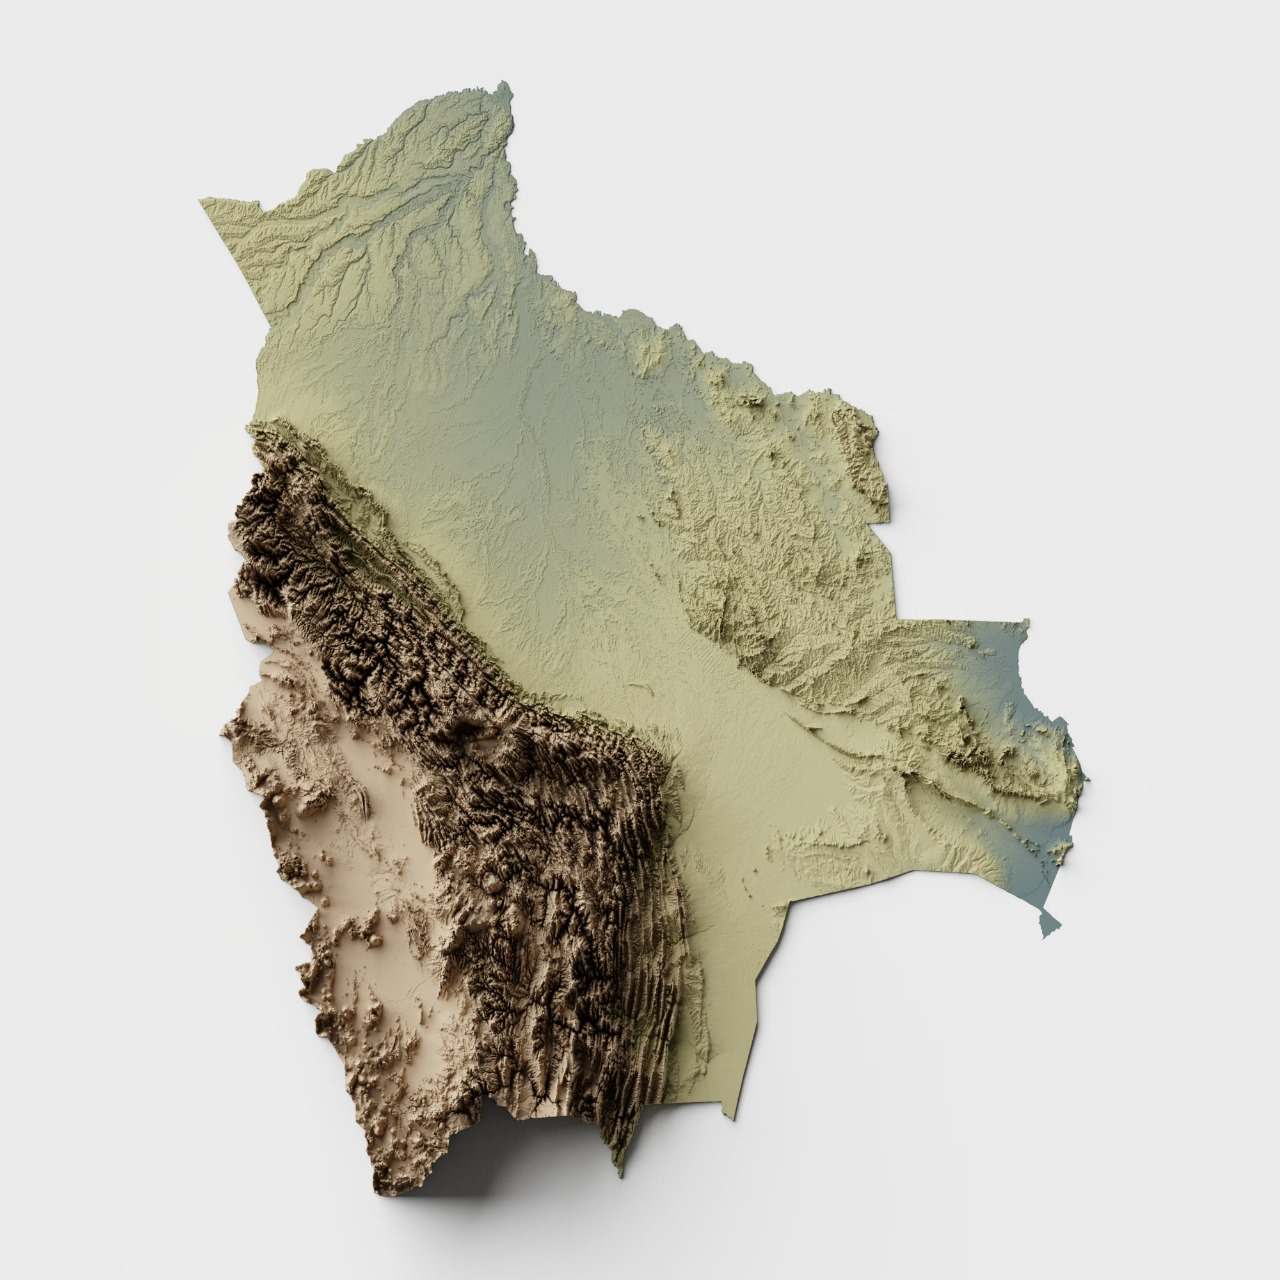
\includegraphics[width=15cm]{bolivian_map}
\end{center}

Bolivia tiene una geografía muy variada, y una de las características principales son sus montañas, los cuales provienen de la cordillera de los Andes que al ingresar al país se divide es dos ramas, cordillera occidental y cordillera oriental, esto fue producido por los diferentes movimientos de las placas tectónicas los cuales son muy recurrentes en el país.
En el cono sur de Cochabamba, a finales de la década de los ’90 se produjo varios terremotos que afectaron gravemente a los municipios de Aiquile, Mizque y Totora. Varias familias quedaron afectadas además que los terremotos en aquella región dejaron grandes pérdidas humanas y económicas.
\\

El siguiente estudio pretende hacer un \textbf{análisis para determinar el nivel de riesgo sísmico que tiene cada región del país} con respecto a los terremotos. Para tal caso se recopilará datos sísmicos por municipios.


\section{Identificación del problema}

\begin{center}
  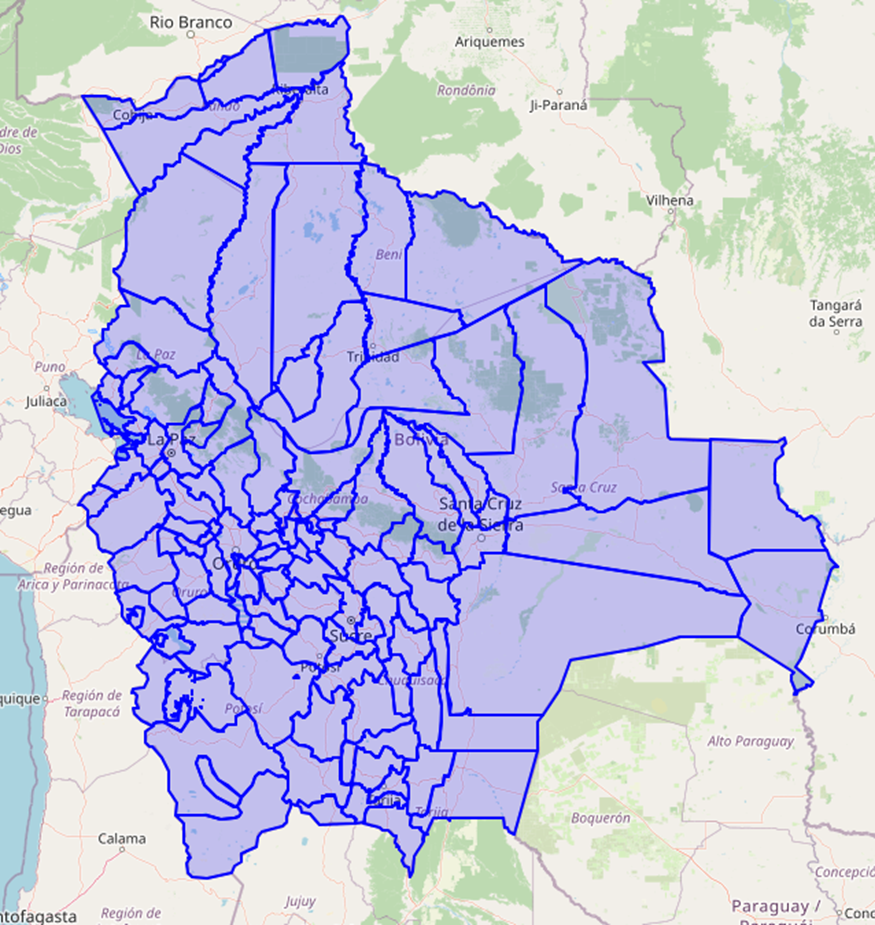
\includegraphics[width=6cm]{bolivia_regiones}
\end{center}


\textbf{Determinar el nivel de riesgo sisimico para cada región de Bolivia.}


\begin{center}
  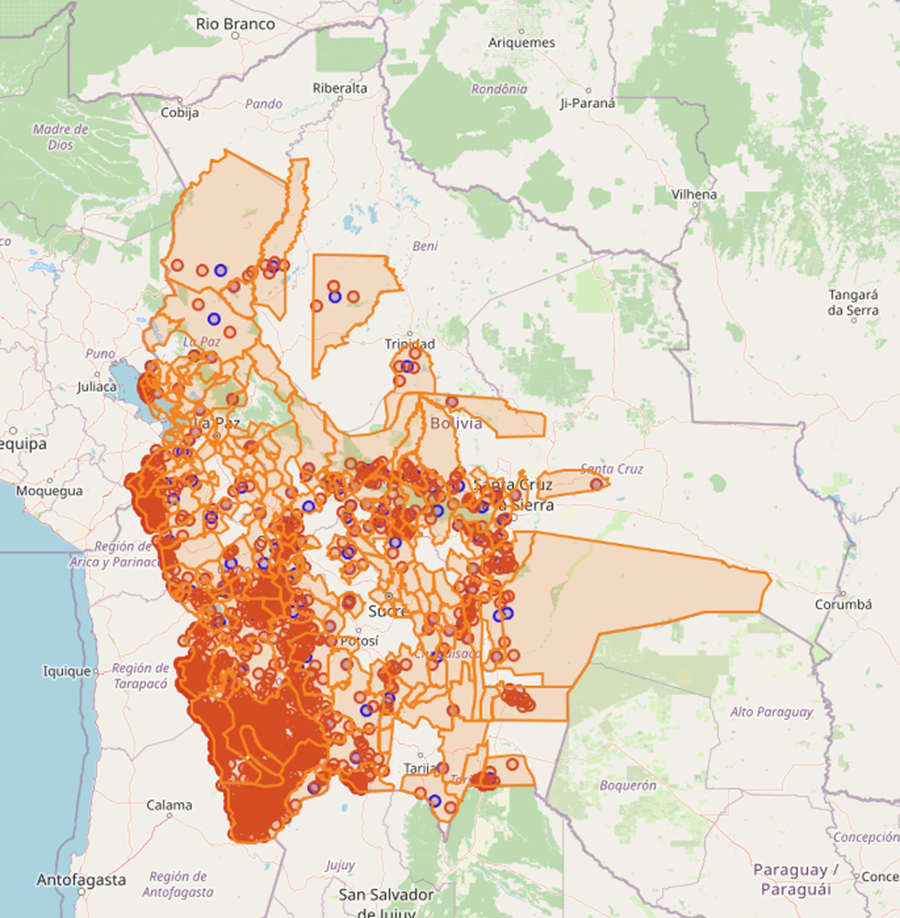
\includegraphics[width=6cm]{bolivia_eq1}
\end{center}


\section{Análisis del problema}

El objetivo principal de este proyecto es clasificar las regiones o municipios de Bolivia según su riesgo sísmico, primeramente, teniendo estos parámetros:

\begin{itemize}
\item\textbf{very\_low} 	= Municipios donde nunca se produjo actividad sísmica.
\item \textbf{low}		= Municipios con menos de 5 registros sísmicos.
\item \textbf{mid}	= Municipios entre 5 – 20 registros sisimicos.
\item \textbf{high}	= Municipios entre 20 – 100 registros sísmicos.
\item \textbf{very\_high}	= Municipios con más de 100 registros sísmicos.
\end{itemize}




\section{Análisis  de los datos}

Para el estudio de datos se seleccionaron las siguientes variables:


\begin{table}[H]
\centering
\begin{tabular}{c c c}
	\hline\hline & \\[-1.5ex]
		\textbf{VARIABLE} &
		\textbf{TIPO DE VARIABLE} &
		\textbf{TABLA ORIGEN}\\ [0.5ex]
	\hline\hline & \\[1.5ex]
		municipality\_code &
		cualitativa & 
		bol\_adm3
  		\\ [1ex]
	\hline & \\[-1.5ex]
department &
cualitativa	&
bol\_adm1
  	\\ [1ex]
	\hline & \\[-1.5ex]
province & cualitativa & bol\_adm2
  	\\ [1ex]
	\hline & \\[-1.5ex]
municipality & cualitativa & bol\_adm3
  	\\ [1ex]
	\hline & \\[-1.5ex]
earthquake\_count & cuantitativa & earthquake\_bol
  	\\ [1ex]
	\hline & \\[-1.5ex]
	
risk & cuantitativa & earthquake\_bol
  	\\ [1ex]
	\hline & \\[-1.5ex]
	
min\_mag & cuantitativa & earthquake\_bol
  	\\ [1ex]
	\hline & \\[-1.5ex]
	
	max\_mag & cuantitativa & earthquake\_bol
  	\\ [1ex]
	\hline & \\[-1.5ex]
	
	avg\_mag & cuantitativa & earthquake\_bol
  	\\ [1ex]
	\hline & \\[-1.5ex]
	
	min\_depth & cuantitativa & earthquake\_bol
  	\\ [1ex]
	\hline & \\[-1.5ex]
	
	max\_depth & cuantitativa & earthquake\_bol
  	\\ [1ex]
	\hline & \\[-1.5ex]
	
	avg\_depth & cuantitativa & earthquake\_bol
  	\\ [1ex]
	\hline & \\[-1.5ex]
	
	min\_sig & cuantitativa & earthquake\_bol
  	\\ [1ex]
	\hline & \\[-1.5ex]
	
	max\_sig & cuantitativa & earthquake\_bol
  	\\ [1ex]
	\hline & \\[-1.5ex]
	
	avg\_sig & cuantitativa & earthquake\_bol
  	\\ [1ex]
	\hline & \\[-1.5ex]
	
	seismic\_centroid & cuantitativa (geo-data) & earthquake\_bol\_detail
  	\\ [1ex]
	\hline & \\[-1.5ex]
	
	seismic\_point & cuantitativa (geo-data) & earthquake\_bol\_detail
  	\\ [1ex]
	\hline & \\[-1.5ex]
	
	municipality\_area & cuantitativa (geo-data) & bol\_adm3
  	\\ [1ex]
	\hline & \\[-1.5ex]

\end{tabular}
\label{table:nonlin}
\end{table}


Todas las variables mencionadas en la tabla son la combinación de unir las siguientes tablas:

\begin{itemize}
\item \textbf{bol\_adm1} (geo-data de los departamentos)
\item \textbf{bol\_adm2} (geo-data de las provincias)
\item \textbf{bol\_adm3} (geo-data de los municipios)
\item \textbf{earthquake\_bol} (información importante sísmica)
\item \textbf{earthquake\_bol\_detail} (geo-data de los puntos sísmicos)
\end{itemize}



Para el objetivo del proyecto, se clasifico a los municipios según su nivel sisimico en los siguientes grupos:

\begin{itemize}
\item \textbf{very\_low} 	0 sismos registrados en un municipio
\item \textbf{low}		[1 - 5] sismos registrados.
\item \textbf{mid}		[5 - 20] sismos registrados.
\item \textbf{high}		[20 - 100] sismos registrados.
\item \textbf{very\_high}	[> 100] sismos registrados.
\end{itemize}


\section{Resultados de las muestras}

\begin{center}
  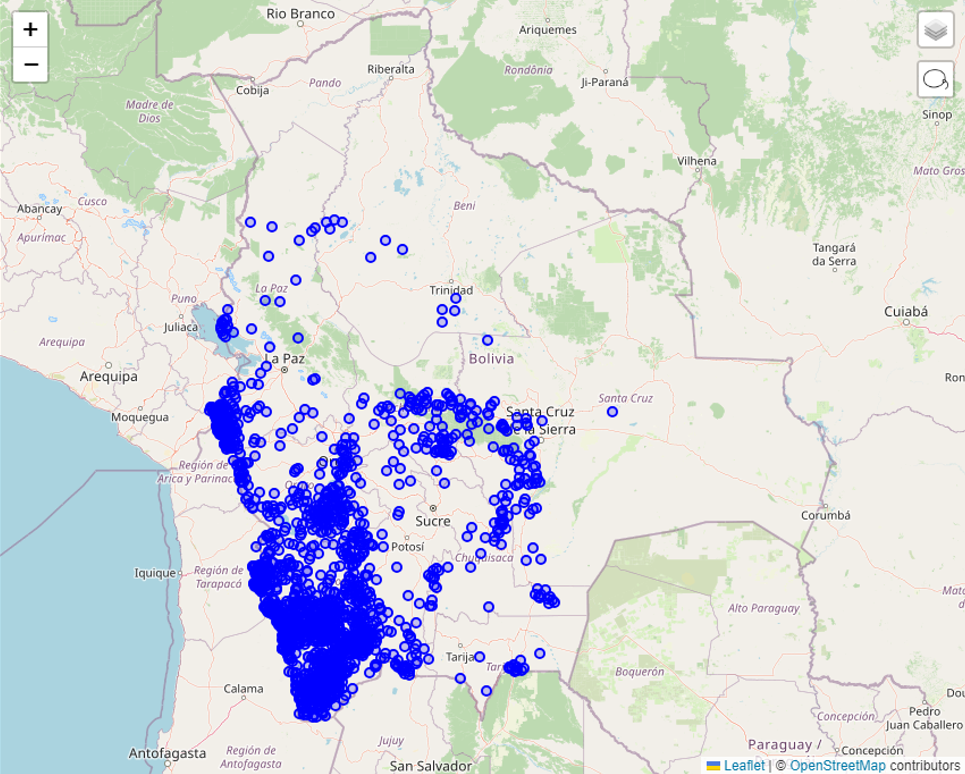
\includegraphics[width=10cm]{bolivia_eq2}
\end{center}

En los resultados del proyecto se pudo clasificar a las regiones en dos grupos, aquellos municipios que tienen actividad sísmica, que mayormente se encuentran en el occidente del país, y los municipios que nos registran actividad sísmica que en su mayoría se encuentran en el oriente.
Existen datos de ciertas regiones donde ya se registran mas de 100 eventos sísmicos contabilizados desde 1920. En total se trabajo con 2006 records para eventos sísmicos los cuales fueron eventos que se suscitaron en 139 municipios de las mas de 340 que existen en el país.






% ----------------------------------------------------------------------
% References
% ----------------------------------------------------------------------

\begin{thebibliography}{00}

\bibitem{b1} Repositorio grupal en Gitlab: big\_data\\
URL: {\url{https://gitlab.com/ramisohj/big_data/-/blob/main/laboratorio_3/docs/laboratorio_3.pdf}}

\bibitem{b1} Repositorio del modelo de identificación de desperdicios: big\_data\\
URL: {\url{https://github.com/AgaMiko/waste-datasets-review}}
\end{thebibliography}


\end{document}